\section{Dijkstra's algorithm}
	Any time the player is training combat, they have to also make a choice about what skill to train. The skill choices are attack, strength, ranged, magic, and defence. Hitpoints is automatically trained regardless of style, and prayer is not generally trained during combat (although it is totally possible). Furthermore, attack options that offer "shared xp" significantly complicate the model since it forces the problem space into xp (which exceeds 10 million) whereas without that only levels are needed (less than 100), as a result it will also be ignored.

	Let's assume a player in a standard loadout (using a dscim within the Nightmare Zone) starts at levels (attack=60, strength=60) and their goal is obtaining (99, 99). The player's first choice is between training to (61, 60) or (60, 61). Repeatedly asking that question all the way to (99, 99) gives the tree-like graph depicted in Fig.~\ref{fig:training_order60}. 


	Since every level exponentially increases the amount of time it takes to train, training one skill results in diminishing returns. Shortest Path algorithms are specially designed to solve this problem, with Dijkstra's algorithm being able to compute exact solutions. The interplay between incremental boosts and longer training times produces optimal solutions like the one shown in Fig.~\ref{fig:training_order_sequence}. This is further illustrated in Fig.~\ref{fig:training_graph}.

	\begin{figure}
		\centering
		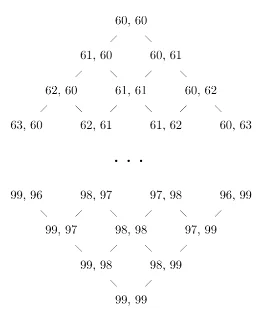
\includegraphics[width=0.5\linewidth]{img/combat/training_order60.png}
		\caption{
			A depiction of the choices the player has to make as they train their attack and strength skills from (60, 60) to (99, 99). Starting at the top, each tier represents a choice to train either attack (right-down) or strength (left-down).
		}
		\label{fig:training_order60}
	\end{figure}

	\begin{figure}
		\centering
		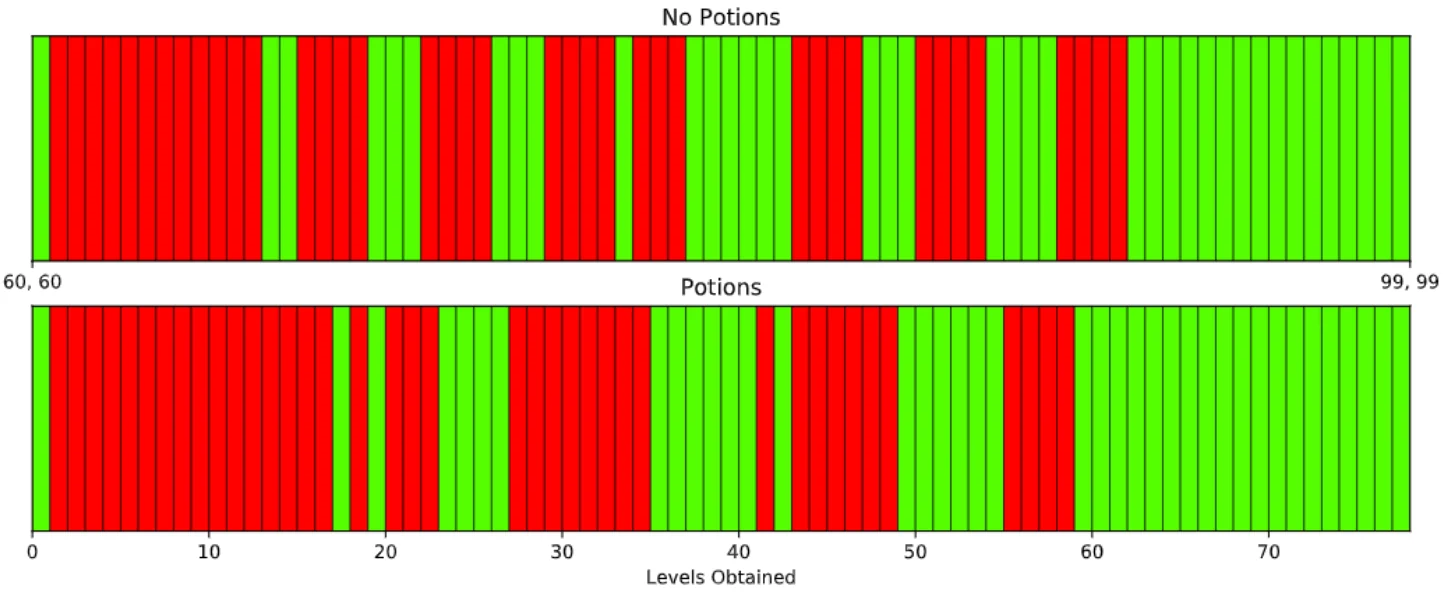
\includegraphics[width=\linewidth]{img/combat/training_order_sequence.png}
		\caption{
			The sequence of training strength (red) and attack (green) for a player both using potions and not. It is clear that starting with strength training is ideal, with the last levels all being attack.
		}
		\label{fig:training_order_sequence}
	\end{figure}

	\begin{figure}
		\centering
		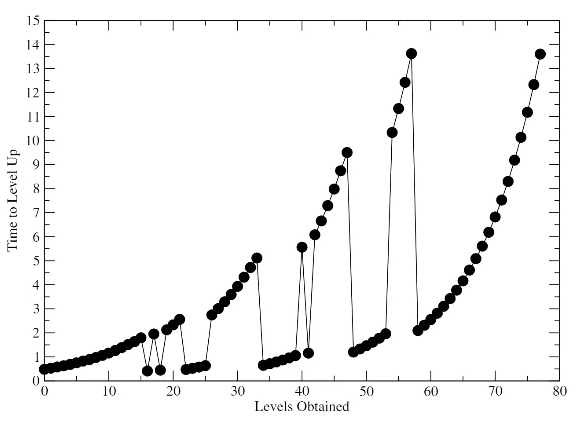
\includegraphics[width=\linewidth]{img/combat/training_graph.png}
		\caption{
			The time taken to level up plotted against the number of levels the player has trained. Two bands clearly emerge which are associated with strength (top) and attack (bottom). The player initially trains strength (driving up the time to level) until about 15 levels are gained, at which point the minor improvement from attack out-competes the large amount of time to get the next strength level. 
		}
		\label{fig:training_graph}
	\end{figure}

	The human player typically optimizes these choices heuristically, and so it is interesting to compare the optimal graph solution with other options. The table below compares different strategies, most notably the optimal solution is only a 0.5\% improvement over simply training strength to 99 then training attack. By contrast, maxing attack first increases training time by 20\%, since the max hit cannot increase. Most players intuitively understand that strength is much more important than attack.

	\begin{table}[h!]
		\centering
		\begin{tabular}{|l|c|c|c|}
		\hline
		\textbf{Strategy} & \textbf{Total Time (h)} & \textbf{Additional Time (h)} & \textbf{\% Improvement} \\
		\hline
		Inverted & 356.6 & 30.1 & 8.4 \\
		\hline
		$(1, 99) \to (99, 99)$ & 328.3 & 1.8 & 0.5 \\
		\hline
		$(99, 1) \to (99, 99)$ & 393.4 & 66.9 & 17 \\
		\hline
		\end{tabular}
		\caption{Comparison of different training orders}
		\label{table:1}
	\end{table}


	The main reason defence training has been omitted is that if defence is trained the player may unlock new armor. So the solution described in the Optimizing Player Equipment chapter is required. At each level, the optimal equipment is determined by set reduction and the experience rates are then calculated. In Fig.~\ref{fig:defence_training} the effect of equipment upgrades is shown.

	\begin{figure}
		\centering
		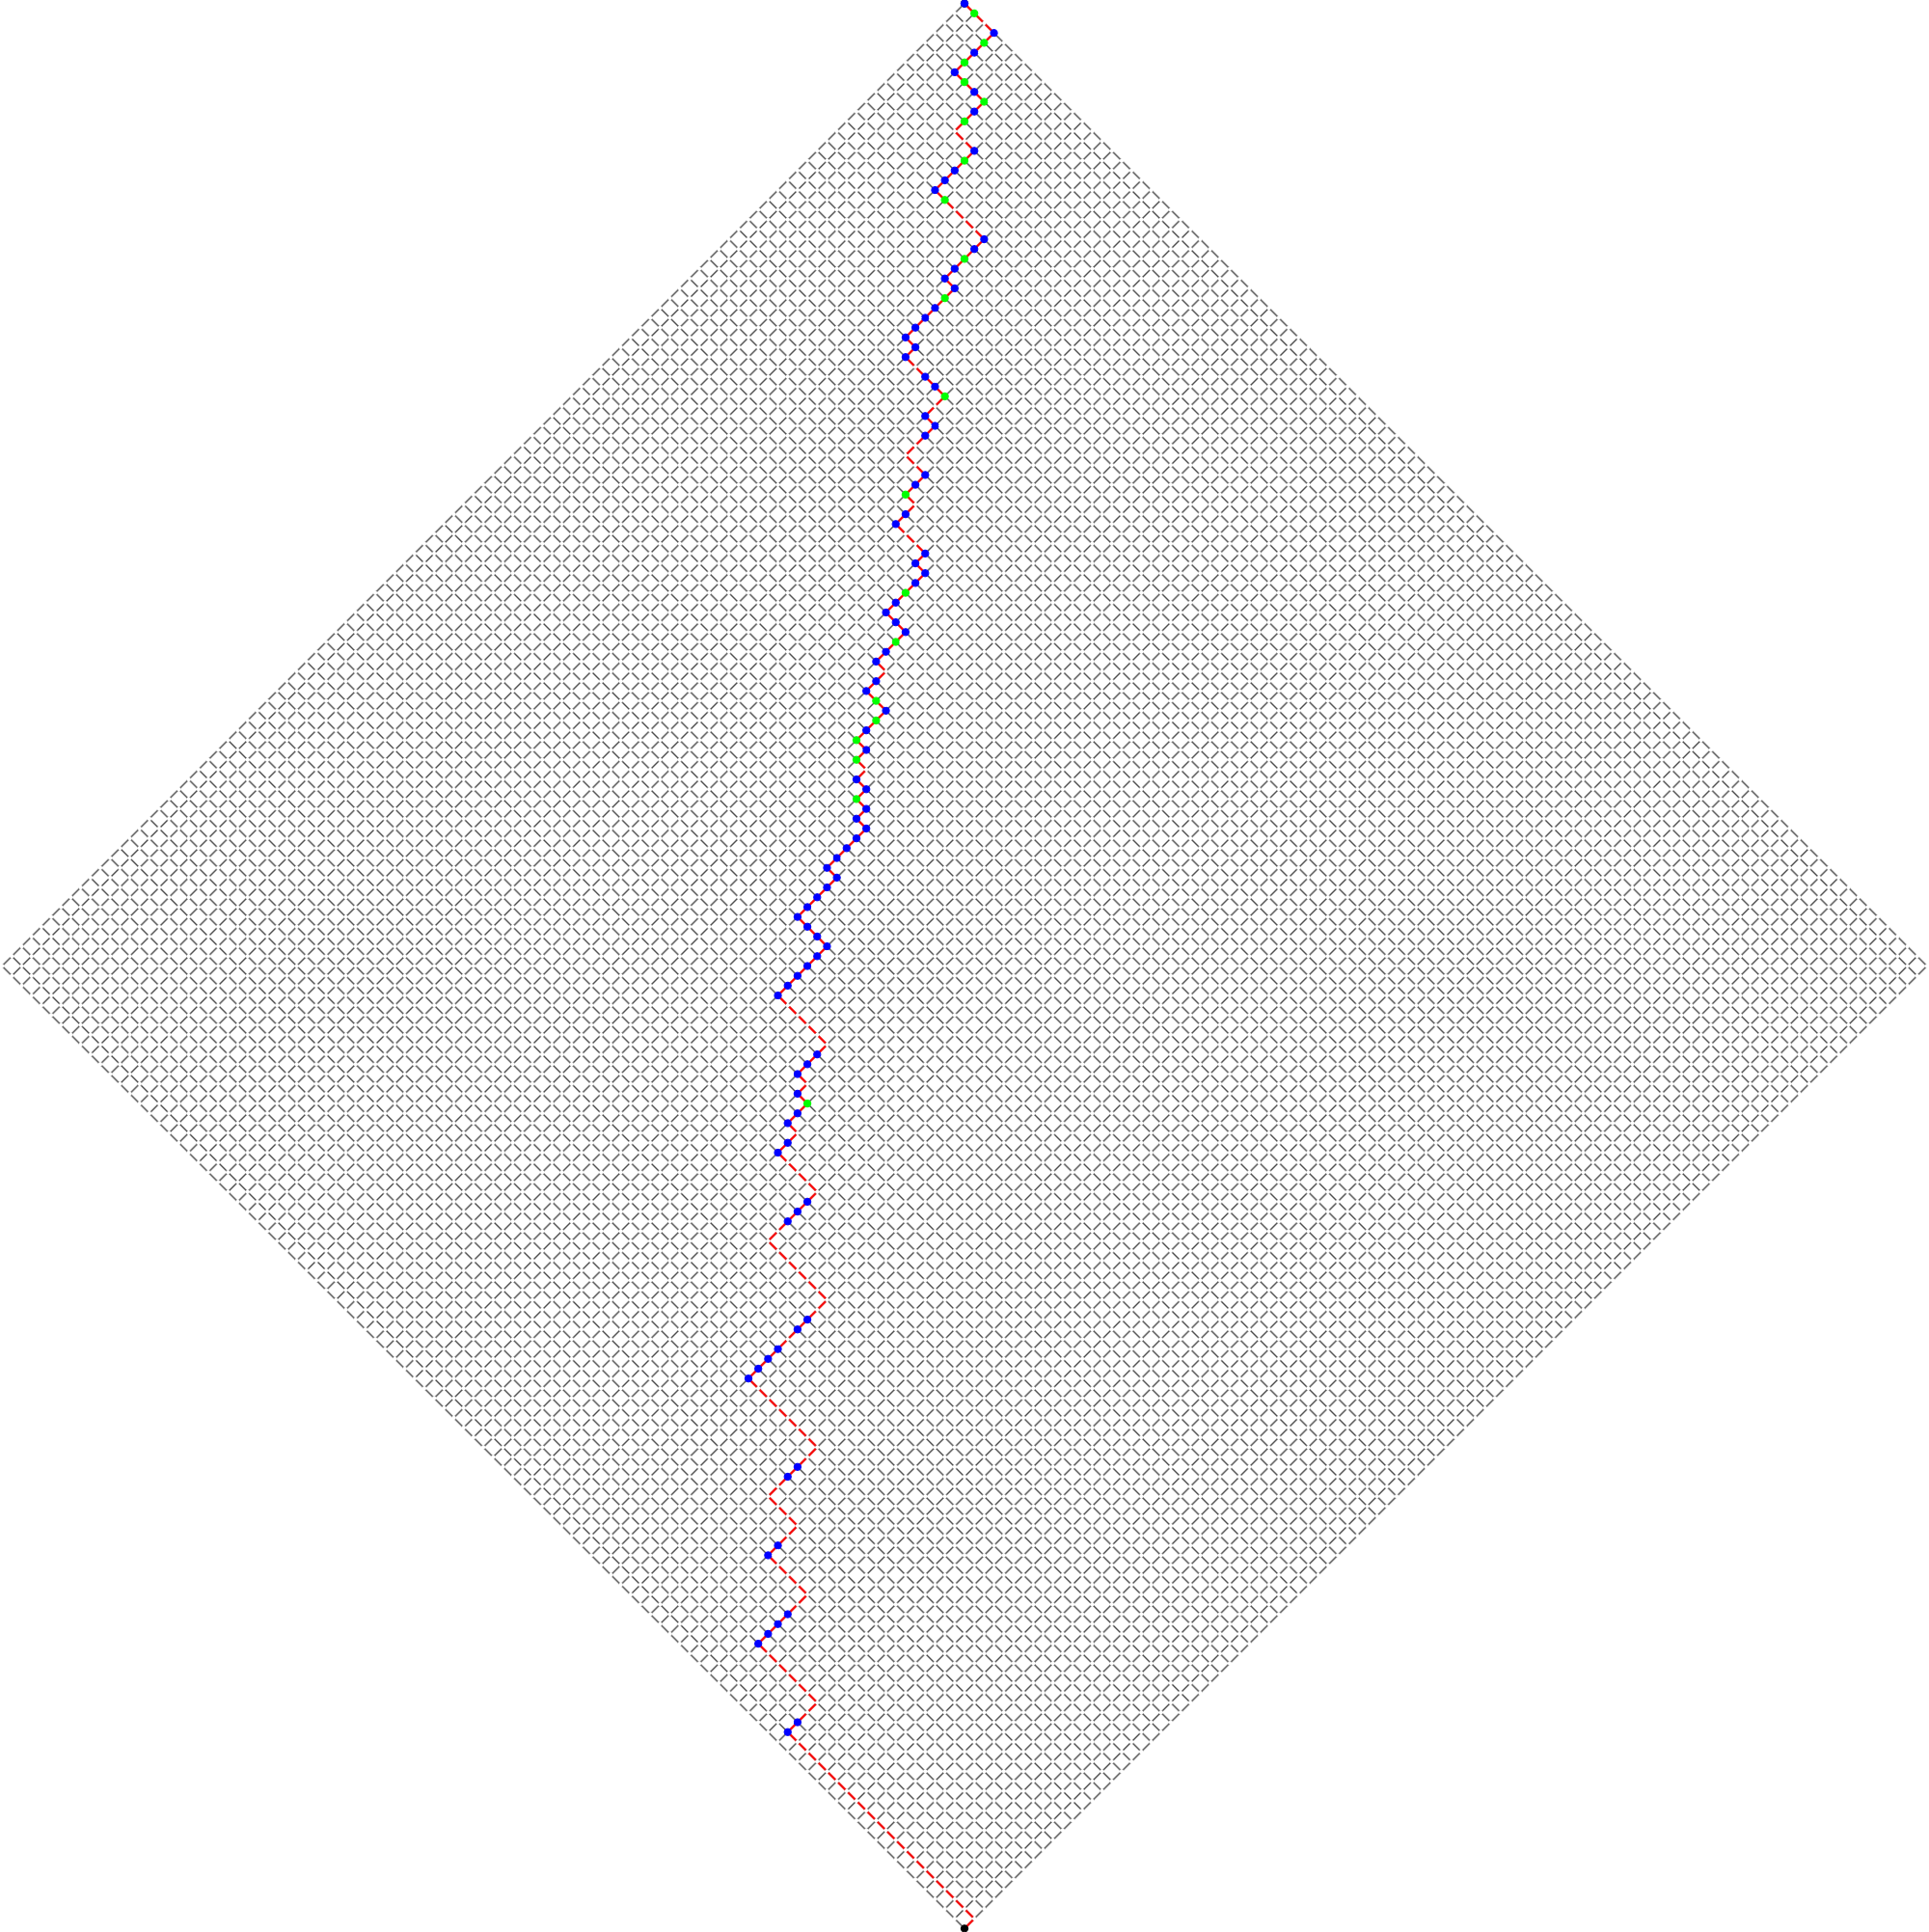
\includegraphics[width=\linewidth]{img/combat/defence_training.png}
		\caption{
			The optimal training order solution from level (1, 1) to (99, 99), while allowing for optimal equipment to be determined at each level. Green nodes indicate that a previously unseen/unused piece of equipment is now being used by the player. Blue nodes indicate that the player changed their gear to something they previously had. The consistent leftward tilt of the training order suggests that keeping your strength $\sim$10\% over your attack level is near-optimal.
		}
		\label{fig:defence_training}
	\end{figure}